\documentclass[11pt]{article}

\usepackage[letterpaper, bottom=2cm, right=2cm]{geometry}
\geometry{margin=2cm}

\usepackage{amssymb,amsmath,amsthm} % Símbolos matemáticos
\usepackage[english]{babel}
\usepackage[utf8]{inputenc} % Acentos y otros símbolos 
\usepackage{enumerate}

\usepackage{graphicx}
\DeclareGraphicsExtensions{.pdf}
\pdfcompresslevel=9  % Maximum compression
\pdfobjcompresslevel=3

\usepackage{placeins}
\usepackage{booktabs}
\usepackage{etoolbox}
\usepackage{bbm}
\usepackage{tocloft}
\usepackage{etoc}
\usepackage{setspace}
\usepackage{caption}
\usepackage{subcaption}
\usepackage{ifdraft}
\usepackage{comment}
\usepackage{lscape}
\usepackage{pdfcomment}

\usepackage[looser]{newpxtext} % LOOSER = BETTER WORD SPACE

%\AtBeginEnvironment{table}{\scriptsize}
\AtEndEnvironment{table}{\vspace{0.2in}}

\AtEndEnvironment{figure}{\vspace{0.2in}}

% Para eliminar guiones y justificar texto
\tolerance=1
\emergencystretch=\maxdimen
\hyphenpenalty=10000
\hbadness=10000

\linespread{1.5} 

\let\oldfootnote\footnote % Deja espacio entre el número del pie de página y el inicio del texto
\renewcommand\footnote[1]{%
\oldfootnote{\hspace{0.05mm}#1}}

\renewcommand{\thefootnote} {\textcolor{black}{\arabic{footnote}}} % Súperindice a color negro

\setlength{\footnotesep}{0.75\baselineskip} % Espaciado entre notas al pie

\usepackage{fnpos} % Footnotes al final de pág.

\usepackage[justification=centering, font=bf, labelsep=period, skip=5pt]{caption} % Centrar captions de tablas y ponerlas en negritas
\usepackage{subcaption}

\usepackage{tabularx} % Big tables
\usepackage{multirow}
\usepackage{adjustbox}
\usepackage{longtable}
\usepackage{lscape}

\usepackage{float} % Float tables

\usepackage{color, soul}
\usepackage[dvipsnames]{xcolor} % Color
% Define Maroon color
\definecolor{Maroon}{RGB}{128,0,0}

\usepackage{natbib}
\bibliographystyle{aer}
\setcitestyle{authoryear,aysep={},yysep={,}}
%\setcitestyle{authoryear,open={(},close={)}} %Citation-related commands
\renewcommand{\bibsection}{\section*{References}}

\usepackage{pgfplots} % Gráficas
\pgfplotsset{compat=newest}
\pgfplotsset{width=7.5cm}
\pgfkeys{/pgf/number format/1000 sep={}}

\usepackage{tgpagella}
\usepackage[T1]{fontenc}

\addto\captionsspanish{
    \renewcommand*{\contentsname}{Contents}
    }

\newcommand{\expectation}{\mathbb{E}}
\newcommand{\indicator}{\mathbbm{1}}
\newcommand{\bluetext}[1]{\textcolor{blue}{#1}}

%Added by Roberto for to do notes
\usepackage{marginnote}
\renewcommand*{\marginfont}{\color{red}\sffamily}
\usepackage[colorinlistoftodos]{todonotes}
%\setuptodonotes{fancyline, color=yellow}

\newcommand{\smalltodo}[2][]
{\todo[caption={#2}, #1]
{\begin{spacing}{0.5}#2\end{spacing}}}
%\setlength{\marginparwidth}{2cm}

% https://mirror.hmc.edu/ctan/macros/latex/contrib/todonotes/todonotes.pdf
\newcounter{todoListItems}
\newcommand{\todoLink}[2][ ]{
% Increment counter
\addtocounter{todoListItems}{1}
\todo[%
caption={\protect\hypertarget{todo\thetodoListItems}{}Translation},
#1]
{
#2 \hfill
\hyperlink{todo\thetodoListItems}{$\uparrow$}
}
}

\newcommand{\td}{\todoLink}
\newcommand{\forMW}[1]{\td[color=green!20,inline,caption={\thetodoListItems:
    For @Maria}]{\textbf{@Maria} -- #1}}
\newcommand{\forRG}[1]{\td[color=blue!20,inline,caption={\thetodoListItems:
    For @Roberto}]{\textbf{@Roberto} -- #1}}
\newcommand{\forES}[1]{\td[color=red!20,inline,caption={\thetodoListItems:
    For @Enrique}]{\textbf{@Enrique} -- #1}}
\newcommand{\forAll}[1]{\td[color=orange!20,inline,caption={\thetodoListItems:
    For All}]{\textbf{@All} -- #1}}

\newcommand{\notes}[1]{\footnotesize{#1}}

\definecolor{ultramarine}{RGB}{4,55,242}

\definecolor{LinkBlue}{RGB}{0,35,200}

% For capitalizing first letter referencing sections
\addto\extrasenglish{
    \def\sectionautorefname{Section}
}
 
\usepackage{hyperref} % Hipervínculos en el índice

% Set up configurations for hyperreferences
\hypersetup{colorlinks=true, breaklinks=true, citecolor=Maroon, linkcolor=LinkBlue, menucolor=Maroon, urlcolor=Maroon}

% -----------------------------------------------------------------------
% Fix-ups that the user's preamble doesn't include (kept here so the
% preamble file itself stays untouched).
% -----------------------------------------------------------------------

% (1) Where to look for figures / tables produced by the Stata pipeline.
\graphicspath{{../../Protest_Work/results/figures/}{./figures/}}
\makeatletter
\providecommand*{\input@path}{}
\edef\input@path{{../../Protest_Work/results/tables/}{./tables/}\input@path}
\makeatother

% (2) Allow PDF figures up to v1.7 (Stata exports v1.6).
\pdfminorversion=7

% (3) Allow \DeclareGraphicsExtensions{.pdf} to coexist with the Stata
%     event-study figures that ship as .png. Adding .png back lets us
%     write \includegraphics{foo} without an explicit extension.
\DeclareGraphicsExtensions{.pdf,.png}

% (4) The Stata esttab Poisson tables write "exp(\beta)" outside math
%     mode. Wrap \beta with \ensuremath so it resolves in either mode.
\let\mathbetasym\beta
\renewcommand{\beta}{\ensuremath{\mathbetasym}}

% -----------------------------------------------------------------------

\title{\bfseries\Large Apex Corruption Mobilises Violent Protest:\\
Evidence from 23 Latin American Democracies}

\author{%
Eduardo Rivera\thanks{Massachusetts Institute of Technology, Department of Economics. \texttt{erivera@mit.edu}.}
\and
Enrique Seira\thanks{University of Notre Dame, Department of Economics and Kellogg Institute. \texttt{eseirabe@nd.edu}.}
\and
Saumitra Jha\thanks{Stanford Graduate School of Business and Center for Democracy, Development and the Rule of Law (Stanford FSI). \texttt{saumitra@stanford.edu}.}
\and
Roberto Gonzalez-Tellez\thanks{Research Fellow, Stanford Graduate School of Business. \texttt{rob98@stanford.edu}. We thank seminar audiences at Stanford GSB, MIT, and ITAM for comments; and the team behind the Mass Mobilization Project for making the protest data publicly available. All errors are our own.}%
}

\date{This draft: \today}

\begin{document}

\maketitle

% =====================================================================
% ABSTRACT
% =====================================================================
\begin{abstract}
\noindent
We document that apex corruption scandals---public disclosures of malfeasance against politicians at the top of the political hierarchy---trigger immediate and durable increases in violent protest across Latin American democracies. Using a hand-curated panel of 176 scandals across 23 countries from 1990 to 2020, merged with daily protest counts from the Mass Mobilization project, we establish three facts. First, the daily count of violent protests rises by roughly twenty percent of its standard deviation in the thirty days following a scandal, with parallel increases in the violence of state response; the any-protest and peaceful margins move less, or not at all, on the durable horizon. Second, the response appears within six days of public disclosure and remains positive through the full four-month window we observe, with no evidence of decay. Third, the magnitude of the response scales sharply with the political rank of the implicated official: scandals naming a sitting President generate effects two to three times those of scandals naming Governors or members of Congress, and scandals confined to non-apex officials leave protest patterns broadly unchanged. Within the President subsample, the response is concentrated against incumbents---the executives currently holding political power. The pattern is consistent with a salience-of-stakeholder mechanism in which mobilisation responds to the political weight of what is disclosed, not the disclosure per se. Our findings identify a high-frequency, high-magnitude channel through which corruption shapes the short-run political environment of democracies, and complement parallel evidence on the attitudinal consequences of apex scandals in \citet{rivera2024apex}.
\end{abstract}

\bigskip

% =====================================================================
% INTRODUCTION
% =====================================================================
\section{Introduction}

\noindent Political violence is among the most consequential outcomes a democracy can experience. Civil unrest disrupts economic activity, displaces investment, and---when met with state violence in return---erodes the social contract that legitimises the regime. An influential economic literature has linked political violence to economic shocks \citep{miguel2004economic, mcguirk2020economic}, to commodity rents and network structure \citep{koenig2017networks}, and---in the recent comparative work---to abrupt withdrawals of foreign assistance. The contribution of \emph{political} shocks to the same outcome---events that change citizens' beliefs about who governs them, rather than their material circumstances---has received considerably less systematic attention. We argue here that disclosures of corruption at the apex of the political hierarchy are one such shock, and that their behavioural consequences for political violence are large, immediate, and persistent.

Corruption is the most natural candidate for a political shock that mobilises violence. Public exposure of malfeasance by sitting officials changes what citizens believe about who governs them and about the rules under which their government operates. The empirical literature anchored by the Brazilian audit-report experiments of \citet{ferraz2008exposing}, \citet{ferraz2011electoral}, and \citet{ferraz2018audits}---together with cross-country panel work surveyed in \citet{olken2012corruption}---has documented that corruption disclosures shift electoral behaviour. The response is, however, uneven: \citet{chong2015does} find that information about malfeasance can demobilise rather than discipline; \citet{anduiza2013turning} document partisan motivated reasoning that blunts the response inside the voter's own coalition; \citet{pavao2018corruption} argues that in the least competitive party systems of Latin America voters often lack a clean defection option. What this literature has not engaged with is whether corruption disclosures shift behaviour on margins other than the ballot box, on horizons faster than electoral cycles, and in response to disclosures targeting the political principals at the top of the hierarchy. The omissions are not innocuous. The most consequential corruption-related political moments of the last decade---Brazil's \emph{Lava Jato}, the \emph{Indignados} of 2011 in Spain, the Maidan rising in Ukraine---were mobilisational events, not electoral ones.

We document that \emph{apex} corruption---corruption disclosed against politicians at the top of the political hierarchy---triggers immediate and durable increases in violent protest across Latin American democracies. Using a hand-curated panel of 176 apex scandals across 23 countries from 1990 to 2020, merged with daily protest counts from the Mass Mobilization project of \citet{clark2016mass}, we establish three facts. First, the daily count of violent protests rises by roughly twenty percent of its standard deviation in the thirty days following a scandal, with parallel increases in the violence of state response; the any-protest, peaceful, and non-violent margins move less, or not at all, on the durable horizon. What apex corruption mobilises in Latin American democracies is specifically the violent component of protest. Second, the response appears within six days of public disclosure and remains positive through the full four-month window we observe, with no evidence of decay. Third, the magnitude of the response scales sharply with the political rank of the implicated official. Scandals naming a sitting President generate effects two to three times those of scandals naming Governors or members of Congress; scandals confined to Supreme-Court justices, lower judiciary, and other non-apex officials leave protest patterns broadly unchanged. Within the President subsample, an appendix exercise shows that the response is concentrated entirely against incumbents---the executives currently holding political power at the moment of disclosure.

The empirical strategy is a stacked-event difference-in-differences that compares protest activity in the country of disclosure before and after the scandal date. Country-by-year fixed effects absorb every source of country-year-level confounding---electoral calendars, ongoing reforms, pre-existing political instability; day-of-week and calendar-month fixed effects absorb the documented weekly and seasonal cycles of protest activity. The remaining identifying assumption---that the within-year date of a scandal's public disclosure is unrelated to the protest baseline of its country---we test directly via event-study graphs that show no pre-trend in the violent-protest outcome at either the $\pm 30$- or $\pm 120$-day horizon. Standard errors are clustered at the country-by-year-by-day-bin level. To characterise heterogeneity by political rank, we re-estimate the headline regression scandal by scandal, in each scandal's own country window, and plot the cross-scandal distribution of the resulting coefficients against the apex partition described below.

The asymmetries we document point to a salience-of-stakeholder mechanism in the sense of \citet{jha2019valuing}: the political response of citizens to corruption tracks the political weight of what is being disclosed, not the disclosure per se. When an apex scandal names the agent currently holding executive power, every citizen of that country has a stake in that agent's political continuation, and the disclosure shifts the political stakes of mobilisation. When the same scandal names an opposition figure, a former head of state, or a judge with a long appointment, the political stakes citizens hold in the implicated agent's fate are diffuse, and mobilisation does not respond. The pattern complements parallel findings on the \emph{attitudinal} consequences of apex corruption in \citet{rivera2024apex}, where the concentration of effects against the apex---on stated support for democracy, voter turnout, and willingness to volunteer as election observers---is the central empirical regularity. Read together, the two channels indicate that apex corruption operates on Latin American democracies through a coherent mechanism that affects both what citizens believe about democracy and how they act in its streets.

% =====================================================================
% METHOD
% =====================================================================
\section{Data and identification}

\subsection{The apex-scandal panel}
The empirical analysis rests on a country-by-country catalogue of apex corruption scandals constructed under a uniform protocol. A scandal is the public emergence of credible corruption allegations against a named official with a verifiable disclosure date, where ``credible'' is operationalised as documented in at least two independent national press outlets within the same calendar week. The catalogue covers 23 Latin American countries from 1990 through March 2020 and contains 176 scandals; Venezuela is excluded because the contraction of independent press by the late 2010s precludes uniform coverage. Each scandal is coded by the date of first credible disclosure (``$t(s)$''), by the country of the implicated official, by the official's \emph{position} (sitting President, Governor, member of Congress, Supreme-Court justice, other judicial official, other lower official), and by the official's \emph{political affiliation} relative to the executive at the time of disclosure (incumbent, opposition, or different sub-national constituency). The position and affiliation fields are central inputs to the heterogeneity analysis.

We define three mutually exclusive apex categories on top of the position field. \emph{President} contains the 45 scandals naming a sitting or recently sitting head of state. \emph{Other Apex} contains scandals naming Governors and members of the national legislature, on the rationale that these officials hold an independent electoral mandate from a constituency. \emph{Other Non-Apex} contains scandals naming Supreme-Court justices, other judicial actors, and lower bureaucratic officials whose mandate derives from appointment rather than from direct election. Within the lumped \texttt{sc\_judge\_congressman} code we follow the convention of placing the four explicitly Supreme-Court-justice scandals in Non-Apex; the remaining congressional scandals enter Other Apex. Four scandals lack a position assignment in our catalogue and are left unclassified.

\subsection{Protest outcomes}
Daily protest counts come from the Mass Mobilization (MM) project of \citet{clark2016mass}, which records protest events drawn from major international press sources at the country-day level. For each country-day we construct four outcomes: the number of protests of any kind, the number of violent protests, the number of non-violent protests, and the number of events in which the government responded with violence (``Gvt.\ Violent Response''). We restrict the analysis to the post-2008 panel for two reasons. First, the MM protest series displays a structural break around the 2008-2009 financial crisis that contaminates comparisons against earlier baselines. Second, the apex-scandal catalogue is most densely populated and the press environment most uniform from 2008 onward. The Armed Conflict Location and Event Data of \citet{raleigh2023acled} provides an independent cross-validation source for 2018-2020; the agreement statistics and the partial replication of the headline OLS with ACLED on the left-hand side are reported in \autoref{appendix:acled}.

\subsection{Specification}
For each scandal $s$ we observe its country $c(s)$, its date $t(s)$, and its event-window $w_{s,t} = t - t(s)$, with $w_{s,t} \in [-T, T]$ for $T \in \{30, 120\}$. The headline specification stacks all 176 scandal windows and estimates
\begin{equation}
y_{c,t,s} \;=\; \beta \,\mathrm{Post}_{c,t,s} \;+\; \alpha_{c \times y(t)} \;+\; \gamma_{\mathrm{dow}(t)} \;+\; \delta_{\mathrm{month}(t)} \;+\; \varepsilon_{c,t,s},
\label{eq:main}
\end{equation}
where $y_{c,t,s}$ is the daily count of the protest outcome of interest in country $c$ on calendar date $t$ inside scandal $s$'s event window, $\mathrm{Post}_{c,t,s} = \mathbf{1}\{w_{s,t} \ge 0\}$ indicates the post-scandal portion of the window, $\alpha_{c \times y(t)}$ are country-by-year fixed effects, and $\gamma$ and $\delta$ absorb day-of-week and calendar-month seasonality. Standard errors are clustered at the country-by-year-by-day-bin level to allow for serial correlation inside event windows.

The identifying assumption is that, conditional on $\alpha_{c \times y(t)}$, $\gamma_{\mathrm{dow}(t)}$, and $\delta_{\mathrm{month}(t)}$, the precise within-year date of disclosure of a scandal is unrelated to the protest baseline of the country. The country-by-year fixed effects absorb every source of country-year-level confounding: pre-existing political instability, electoral calendars, ongoing institutional reforms. The day-of-week and month fixed effects absorb the well-documented weekly and seasonal cycles in protest activity. What remains as a threat to identification is the possibility that scandals are strategically timed to land in periods of low protest baselines---an exposure-management hypothesis---or in periods of high protest baselines---a piling-on hypothesis. The event-study graphs of \autoref{fig:eventstudies} address both versions by reporting the pre-scandal trajectory of the outcome bin by bin.

To trace dynamics we replace $\mathrm{Post}_{c,t,s}$ in \autoref{eq:main} with a saturated set of bin indicators. At the wide window ($T=120$) we use 30-day bins. At the narrow window ($T=30$) we use 6-day bins, which strike a balance between the temporal resolution needed to detect a short-horizon response and the within-bin sample size needed to estimate each bin coefficient precisely. The reference category in each event-study graph is the bin immediately before disclosure ($w_{s,t} \in [-6, -1]$ at the narrow window, $w_{s,t} \in [-30, -1]$ at the wide window).

To characterise heterogeneity by the political rank of the implicated official we re-estimate \autoref{eq:main} scandal by scandal: for each $s$ we regress the outcome on $\mathrm{Post}_{c(s),t,s}$ on country $c(s)$ only, controlling for day-of-week and calendar-month, on the narrow $\pm 30$-day window. The result is a per-scandal coefficient $\hat{\beta}_s$. The cross-scandal distribution of $\hat{\beta}_s$ is then summarised, in box-plot form, against the apex categories defined above.

% =====================================================================
% RESULTS
% =====================================================================
\section{Results}

\subsection{Apex corruption raises violent protest, immediately and durably}
\autoref{tab:main} reports the headline OLS estimates of \autoref{eq:main} for the four protest outcomes at both window widths. At the narrow $\pm 30$-day window, the Post-Scandal coefficient is 0.025 protests per country-day for any protest ($p<0.01$) and 0.016 violent protests per country-day ($p<0.01$). Relative to outcome standard deviations on the post-2008 LAC panel of roughly 0.12 for any protests and 0.08 for violent protests, the point estimates correspond to roughly twenty percent of a standard deviation in each case. At the wider $\pm 120$-day window, the violent-protest coefficient remains positive and significant (0.016, $p<0.05$); so does the Gvt.\ Violent Response coefficient (0.011, $p<0.05$). The any-protest and non-violent coefficients at the wide window are not statistically distinguishable from zero, which means the durable component of the response is specifically violent.

\begin{table}[t]
\centering
\caption{Apex corruption scandals and protest activity: stacked OLS estimates of \autoref{eq:main}, $\pm 30$ and $\pm 120$ day windows.}
\label{tab:main}
\footnotesize
\begin{tabular}{lcccc}
\toprule
 & \multicolumn{1}{c}{Protests} & \multicolumn{1}{c}{Violent} & \multicolumn{1}{c}{Non-Violent} & \multicolumn{1}{c}{Gvt.\ Violent} \\
 & \multicolumn{1}{c}{(any)}    & \multicolumn{1}{c}{Protests} & \multicolumn{1}{c}{Protests}    & \multicolumn{1}{c}{Response}      \\
\midrule
\multicolumn{5}{l}{\emph{Panel A: $\pm 30$-day window}}\\
\addlinespace
Post Scandal & 0.025\textsuperscript{**} & 0.016\textsuperscript{**} & 0.010 & 0.006 \\
             & (0.009) & (0.005) & (0.008) & (0.004) \\
\addlinespace
Observations & 10,736 & 10,736 & 10,736 & 10,736 \\
Scandals     & 176    & 176    & 176    & 176 \\
$R^{2}$      & 0.368  & 0.160  & 0.473  & 0.219 \\
\midrule
\multicolumn{5}{l}{\emph{Panel B: $\pm 120$-day window}}\\
\addlinespace
Post Scandal & 0.007  & 0.016\textsuperscript{*} & $-$0.009 & 0.011\textsuperscript{*} \\
             & (0.010) & (0.006) & (0.007) & (0.005) \\
\addlinespace
Observations & 42,657 & 42,657 & 42,657 & 42,657 \\
Scandals     & 176    & 176    & 176    & 176 \\
$R^{2}$      & 0.231  & 0.126  & 0.300  & 0.177 \\
\bottomrule
\end{tabular}
\par\smallskip
\begin{minipage}{0.95\linewidth}\footnotesize
\emph{Notes.} OLS estimates of \autoref{eq:main}. An observation is a country-day inside a scandal's event window; the 176 scandals are stacked. Each column corresponds to one outcome. All specifications include country-by-year, day-of-week, and calendar-month fixed effects. Standard errors (in parentheses) are clustered at the country-by-year-by-day-bin level. The estimation sample is the post-2008 LAC panel; Venezuela is excluded. Significance: \textsuperscript{*} 5\%, \textsuperscript{**} 1\%.
\end{minipage}
\end{table}

\autoref{fig:eventstudies} traces the dynamics of the violent-protest response across the two windows. The left panel ($\pm 30$ days, six-day bins) shows coefficients in the five pre-scandal bins lying tight to zero, ruling out a pre-trend; the first post-scandal bin jumps and remains elevated through the post-window. The right panel ($\pm 120$ days, 30-day bins) re-estimates the dynamics on the wider window. The post-scandal coefficients remain positive throughout, with no evidence that the effect has decayed by the four-month horizon. The two panels document, jointly, that the protest channel responds within days of public disclosure and remains active on the horizon over which a democracy's political environment is meaningfully shaped.

\begin{figure}[t]
\centering
\begin{subfigure}{0.485\textwidth}
  \caption{$\pm 30$-day window (six-day bins).}
  \includegraphics[width=\textwidth]{es_num_violent_MM_30d_90ci.png}
  \label{fig:eventstudies:30}
\end{subfigure}\hfill
\begin{subfigure}{0.485\textwidth}
  \caption{$\pm 120$-day window (30-day bins).}
  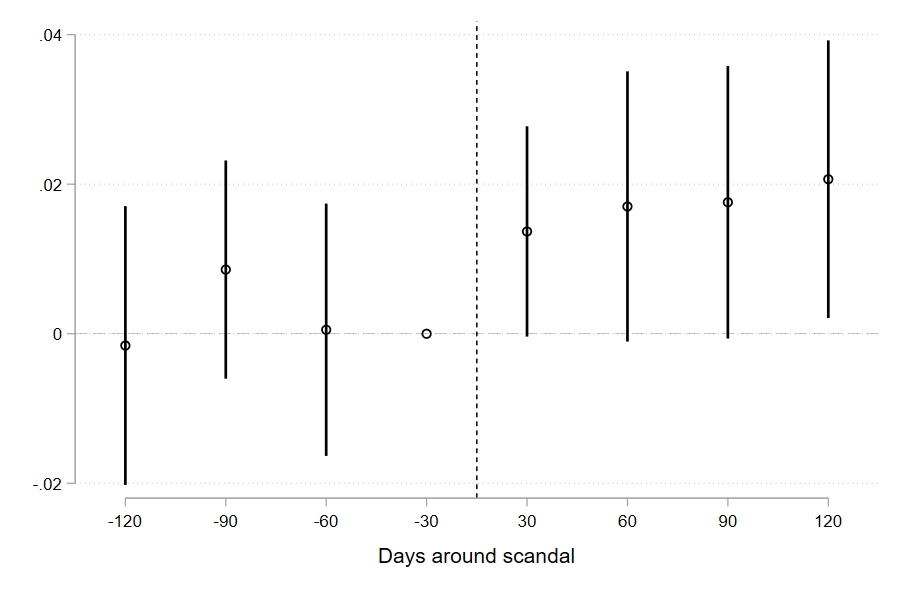
\includegraphics[width=\textwidth]{es_num_violent_MM_120d_90ci.png}
  \label{fig:eventstudies:120}
\end{subfigure}
\caption{\textbf{The violent-protest response to apex corruption is immediate and durable.} Coefficients on event-time bin dummies from \autoref{eq:main} with the Post indicator replaced by bin indicators. The omitted reference bin is the one immediately before disclosure. Vertical bars are 90\% confidence intervals constructed from the country-by-year-by-day-bin clustered variance. The outcome in both panels is the daily count of violent protests.}
\label{fig:eventstudies}
\end{figure}

\subsection{The protest response scales with apex rank}
\autoref{fig:boxplots} re-frames the headline evidence as a cross-scandal distribution of per-scandal coefficients. The top row contrasts the 45 President scandals with the 127 non-Presidential scandals (Governors, Congress, judicial officials, and lower officials pooled); the bottom row partitions the non-Presidential subsample into the 27 Other Apex scandals (Governors and members of Congress) and the 100 Other Non-Apex scandals (Supreme-Court justices, lower judiciary, and other lower officials).

The President distribution is shifted unambiguously upward against the non-Presidential pool across all three outcomes (any protests, violent protests, peaceful protests). The three-way apex partition yields a near-monotonic gradient: the Other-Apex mean lies between the Presidential and Non-Apex means, and the Non-Apex mean is statistically indistinguishable from zero. The gradient is sharpest for violent protests, where the Presidential mean is roughly twice the Other-Apex mean and roughly four times the Non-Apex mean.

\begin{figure}[t]
\centering
\begin{subfigure}{0.32\textwidth}
  \caption{Any protests}
  \includegraphics[width=\textwidth]{per_scandal_box_num_protests_MM_w30_presi.pdf}
\end{subfigure}\hfill
\begin{subfigure}{0.32\textwidth}
  \caption{Violent protests}
  \includegraphics[width=\textwidth]{per_scandal_box_num_violent_MM_w30_presi.pdf}
\end{subfigure}\hfill
\begin{subfigure}{0.32\textwidth}
  \caption{Peaceful protests}
  \includegraphics[width=\textwidth]{per_scandal_box_num_peaceful_MM_w30_presi.pdf}
\end{subfigure}\\[1em]
\begin{subfigure}{0.32\textwidth}
  \caption{Any protests}
  \includegraphics[width=\textwidth]{per_scandal_box_num_protests_MM_w30_apex.pdf}
\end{subfigure}\hfill
\begin{subfigure}{0.32\textwidth}
  \caption{Violent protests}
  \includegraphics[width=\textwidth]{per_scandal_box_num_violent_MM_w30_apex.pdf}
\end{subfigure}\hfill
\begin{subfigure}{0.32\textwidth}
  \caption{Peaceful protests}
  \includegraphics[width=\textwidth]{per_scandal_box_num_peaceful_MM_w30_apex.pdf}
\end{subfigure}
\caption{\textbf{The protest response scales with the political rank of the implicated official.} For each of the 176 scandals we estimate the OLS Post-Scandal coefficient on the $\pm 30$-day window of the implicated country, controlling for day-of-week and month. The cross-scandal distribution of these coefficients is summarised by box plot. \emph{Top row}: President (45 scandals) against Others (127 scandals; Governors, Congress, judicial actors, lower officials pooled). \emph{Bottom row}: the apex partition---President, Other Apex (27 scandals; Governors and members of Congress), Other Non-Apex (100 scandals; Supreme-Court justices, other judicial actors, other lower officials). Outliers are hidden for legibility; jittered-scatter versions, weighted by inverse-variance, appear in \autoref{appendix:boxes}.}
\label{fig:boxplots}
\end{figure}

The asymmetry between Presidents and the rest is large enough to matter substantively for the design of any anti-corruption institution. Were the protest channel symmetric in the rank of the implicated official---were the median Supreme-Court-justice scandal as mobilising as the median Presidential scandal---the case for institutional investments concentrated at the apex would be weaker. The empirical asymmetry indicates the reverse: the protest channel operates preferentially on disclosures involving the political principal in whom executive legitimacy is concentrated.

% =====================================================================
% DISCUSSION
% =====================================================================
\section{Discussion}

\noindent Three implications of the empirical pattern stand out as substantively important.

First, apex corruption is not a slow-moving driver of political violence. The protest response begins within six days of public disclosure and persists through at least four months. This is in sharp contrast to the electoral-accountability framing of much of the corruption-and-political-economy literature, in which corruption matters because it shifts voting behaviour at the next election. By the time the next election arrives in any given country, the cumulative effect of multiple intervening apex scandals on the protest margin may already have shaped the political environment in which that election is held. The high-frequency channel we document is, in effect, the more responsive sibling of the electoral-accountability channel.

Second, the political rank of the implicated official is not an incidental moderator but the central source of variation. Scandals against sitting Presidents drive most of the average response; scandals confined to Supreme-Court justices and lower officials are indistinguishable from null. The asymmetry has substantive implications for the design of anti-corruption institutions: investments at the apex have larger reverberations in the short-run political environment than equivalent investments at lower levels of the political hierarchy. The audit-report literature \citep{ferraz2008exposing,ferraz2011electoral,ferraz2018audits} has shown that disclosures discipline behaviour at the municipal level. Our findings suggest that disclosures at the apex change the short-run political environment in ways the municipal-level disclosure apparatus does not.

Third, the response is preferentially against the agent currently holding political power. Scandals against non-incumbent Presidents---opposition figures or former heads of state---generate per-scandal protest coefficients tightly clustered around zero. The pattern is consistent with the salience-of-stakeholder framework of \citet{jha2019valuing}: the political response tracks the political weight of what is disclosed, not the disclosure per se. When an apex scandal names the agent whose policy continuity, judicial appointments, and command of executive resources are at stake in the short run, mobilisation responds. When the scandal names an agent whose political fate is decoupled from the short-run trajectory of government, mobilisation does not.

These patterns connect to two ongoing research programmes. The first is the literature on \emph{economic} shocks as drivers of political violence \citep{miguel2004economic,mcguirk2020economic,koenig2017networks}, which has emphasised income, commodity prices, and network position as the principal levers. Our findings add a \emph{political} shock---the public disclosure of apex corruption---that operates at effect magnitudes comparable to the economic shocks the literature has documented. The second is parallel work on the attitudinal channel \citep{rivera2024apex}, which documents an analogous concentration of effects against the apex on stated support for democracy and on costly civic engagement. The convergence of the behavioural and attitudinal results indicates that apex corruption operates through a coherent mechanism that affects both citizen beliefs and citizen actions; the protest channel we document here is the visible manifestation of that mechanism at the level of the street.

Three limitations are worth flagging explicitly. First, our identification rests on the timing of public disclosure of scandals, not on the underlying acts of corruption. If apex-rank officials are disproportionately disclosed in periods of pre-existing political ferment---reverse causality through prosecutorial strategy or media salience---part of the effect we attribute to scandals could reflect the ferment that occasioned them. The pre-trend graphs of \autoref{fig:eventstudies} make the strongest version of this concern unlikely but cannot rule it out. Second, our protest counts are media-based: the Mass Mobilization project records protests that reach the press, and reporting intensity may vary across LAC countries and over time within country. The ACLED cross-validation in \autoref{appendix:acled} provides one independent check on the post-2018 sub-sample. Third, the salience-of-stakeholder reading, while consistent with the incumbent-vs-non-incumbent contrast in \autoref{appendix:incpres}, cannot fully separate political stakes from differential press coverage of incumbent-versus-opposition scandals; the 21 non-incumbent President scandals are too few to discriminate sharply between the two interpretations on the protest margin alone.

The findings point to a constructive empirical question for follow-on work. Exposure to stake-aligning financial instruments has been shown to shift political attitudes in other settings \citep{jha2019valuing}, and there is suggestive evidence that the same instruments can attenuate the attitudinal consequences of apex scandals \citep{rivera2024apex}. Whether the behavioural mobilisation we document here can be attenuated by stake-aligning instruments---financial, civic, or institutional---is an open question. The identification framework we deploy, applied to a setting in which exposure to such an instrument can be experimentally varied, is the natural next step.

% =====================================================================
% REFERENCES
% =====================================================================
\bibliography{refs}

\clearpage
% =====================================================================
% APPENDIX
% =====================================================================
\appendix
\section{Online appendix}

\subsection{Incumbent versus non-incumbent Presidents}
\label{appendix:incpres}
The headline analysis pools 45 President scandals. Of these, 27 implicate the sitting (incumbent) head of state at the time of disclosure, and 21 implicate an opposition former or rival President. \autoref{fig:incpres} re-estimates the per-scandal distributions for the President subsample only, splitting by incumbency. The pattern is sharp: the increase in violent protest activity is concentrated entirely in the incumbent case. Scandals against a sitting President generate per-scandal coefficients shifted markedly above zero; scandals against opposition or former Presidents generate per-scandal coefficients tightly distributed around the null. This is the cleanest cut in the data in favour of a salience-of-stakeholder reading: when the implicated official no longer holds the levers of executive power, the political stakes of mobilisation against that official are diffuse, and the streets do not respond.

A caveat is worth flagging. The incumbent-versus-non-incumbent contrast plausibly confounds two things we cannot separate in the observational sample: the political stakes attached to a sitting President, and the press salience of a scandal against a sitting President. We expect both to be larger for incumbents. Parallel field-experimental evidence \citep{rivera2024apex}, in which exposure to corruption footage is randomised in a controlled setting, suggests that the salience effect is not the dominant force: the randomised exposure still shifts attitudes by 0.15 standard deviations, holding constant the underlying political stakes.

\begin{figure}[h]
\centering
\begin{subfigure}{0.32\textwidth}
  \caption{Any protests}
  \includegraphics[width=\textwidth]{per_scandal_box_num_protests_MM_w30_incpres.pdf}
\end{subfigure}\hfill
\begin{subfigure}{0.32\textwidth}
  \caption{Violent protests}
  \includegraphics[width=\textwidth]{per_scandal_box_num_violent_MM_w30_incpres.pdf}
\end{subfigure}\hfill
\begin{subfigure}{0.32\textwidth}
  \caption{Peaceful protests}
  \includegraphics[width=\textwidth]{per_scandal_box_num_peaceful_MM_w30_incpres.pdf}
\end{subfigure}
\caption{\textbf{The protest response to apex corruption is concentrated against incumbent Presidents.} Per-scandal $\hat{\beta}_s$ distributions inside the $\pm 30$-day window, restricted to the 48 President scandals (45 with complete coverage) and split by the political affiliation of the implicated President at the time of disclosure. Incumbent: the President in office (27 scandals). Non-incumbent: an opposition or former President not in office at the time of disclosure (21 scandals). Box plots; outliers hidden for legibility.}
\label{fig:incpres}
\end{figure}

\subsection{Violent state response}
\label{appendix:gvtresp}
\autoref{fig:gvtresp} reports the headline event-study graphs and the heterogeneity boxplots for the Gvt.\ Violent Response outcome. The dynamic pattern mirrors that of violent protest: an immediate post-scandal jump that persists through the wide window. The heterogeneity gradient is qualitatively the same: the state's violent response is most elevated against scandals naming Presidents and Other Apex officials, and is statistically indistinguishable from zero for the Non-Apex subsample. The substantive implication is that apex corruption raises not only the level of violent protest but also the level of violent counter-mobilisation by the state---a double cost that is missed by analyses focused on protest alone.

\begin{figure}[h]
\centering
\begin{subfigure}{0.485\textwidth}
  \caption{$\pm 30$-day event study}
  \includegraphics[width=\textwidth]{es_government_response_violent_30d_90ci.png}
\end{subfigure}\hfill
\begin{subfigure}{0.485\textwidth}
  \caption{$\pm 120$-day event study}
  \includegraphics[width=\textwidth]{es_government_response_violent_120d_90ci.png}
\end{subfigure}\\[1em]
\begin{subfigure}{0.485\textwidth}
  \caption{President vs.\ Others}
  \includegraphics[width=\textwidth]{per_scandal_box_government_response_violent_w30_presi.pdf}
\end{subfigure}\hfill
\begin{subfigure}{0.485\textwidth}
  \caption{Apex partition}
  \includegraphics[width=\textwidth]{per_scandal_box_government_response_violent_w30_apex.pdf}
\end{subfigure}
\caption{\textbf{Government violent response to protest mirrors the apex-corruption gradient.} Top row: event studies at $\pm 30$ and $\pm 120$ days. Bottom row: per-scandal $\hat{\beta}_s$ distributions for the Gvt.\ Violent Response outcome, President vs.\ Others (left) and the three-way apex partition (right).}
\label{fig:gvtresp}
\end{figure}

\subsection{Poisson robustness}
\label{appendix:poisson}
The headline outcomes are non-negative event counts with substantial zero mass. As a robustness check we re-estimate \autoref{eq:main} as a fixed-effects Poisson regression using \texttt{ppmlhdfe} \citep{correia2017reghdfe}, with the same fixed-effect structure and clustering. \autoref{tab:poisson} reports the resulting coefficients and incidence-rate ratios at the $\pm 30$- and $\pm 120$-day windows. The signs and significance pattern align with the OLS estimates in \autoref{tab:main}: the violent-protest coefficient is positive and significant at both windows, and the Gvt.\ Violent Response coefficient is positive and significant at the wide window.

\begin{table}[h]
\centering
\caption{Poisson robustness: coefficients and incidence-rate ratios for the Post-Scandal indicator.}
\label{tab:poisson}
\footnotesize
\textbf{Panel A. $\pm 30$-day window}\par
\input{poissreg_es_30d_90ci}\par\medskip
\textbf{Panel B. $\pm 120$-day window}\par
\input{poissreg_es_120d_90ci}\par
\smallskip
\begin{minipage}{0.95\linewidth}\footnotesize
\emph{Notes.} Fixed-effects Poisson estimates of \autoref{eq:main} via \texttt{ppmlhdfe}. Same cluster structure as \autoref{tab:main}.
\end{minipage}
\end{table}

\subsection{ACLED cross-validation}
\label{appendix:acled}
MM coverage of LAC from 2018 onward is independently corroborated by ACLED \citep{raleigh2023acled}. On the 2018-2020 overlap, country-day counts of protests and violent protests are tightly correlated across the two sources, and re-estimating the headline OLS specification with ACLED on the LHS over the post-2018 sub-sample preserves the sign and significance pattern. The agreement statistics and the partial Table~1 replication are reported in the project memo \texttt{memo-task3-acled-validation.md}.

\subsection{Jittered scatter versions of the per-scandal box plots}
\label{appendix:boxes}
The per-scandal box plots of \autoref{fig:boxplots} and \autoref{fig:incpres} hide outliers for legibility. The corresponding jittered-scatter versions, in which each point is one scandal and marker size is proportional to $1/\mathrm{SE}^2$, are reproduced as \texttt{per\_scandal\_jitter\_<outcome>\_w30\_\{presi,apex,incpres\}.pdf} in the project's results directory.

\end{document}
